%%%%%%%%%%%%%%%%%%%%%%%%%%%%%%%%%%%%%%%%%
% Wenneker Assignment
% LaTeX Template
% Version 2.0 (12/1/2019)
%
% This template originates from:
% http://www.LaTeXTemplates.com
%
% Authors:
% Vel (vel@LaTeXTemplates.com)
% Frits Wenneker
%
% License:
% CC BY-NC-SA 3.0 (http://creativecommons.org/licenses/by-nc-sa/3.0/)
% 
%%%%%%%%%%%%%%%%%%%%%%%%%%%%%%%%%%%%%%%%%

%----------------------------------------------------------------------------------------
%	PACKAGES AND OTHER DOCUMENT CONFIGURATIONS
%----------------------------------------------------------------------------------------

\documentclass[11pt]{scrartcl} % Font size

%%%%%%%%%%%%%%%%%%%%%%%%%%%%%%%%%%%%%%%%%
% Wenneker Assignment
% Structure Specification File
% Version 2.0 (12/1/2019)
%
% This template originates from:
% http://www.LaTeXTemplates.com
%
% Authors:
% Vel (vel@LaTeXTemplates.com)
% Frits Wenneker
%
% License:
% CC BY-NC-SA 3.0 (http://creativecommons.org/licenses/by-nc-sa/3.0/)
% 
%%%%%%%%%%%%%%%%%%%%%%%%%%%%%%%%%%%%%%%%%

%----------------------------------------------------------------------------------------
%	PACKAGES AND OTHER DOCUMENT CONFIGURATIONS
%----------------------------------------------------------------------------------------

\usepackage{amsmath, amsfonts, amsthm} % Math packages

\usepackage{listings} % Code listings, with syntax highlighting

\usepackage[english]{babel} % English language hyphenation

\usepackage{graphicx} % Required for inserting images
\graphicspath{{figures/}{./}{../plots/}} % Specifies where to look for included images (trailing slash required)

\usepackage{booktabs} % Required for better horizontal rules in tables

\numberwithin{equation}{section} % Number equations within sections (i.e. 1.1, 1.2, 2.1, 2.2 instead of 1, 2, 3, 4)
\numberwithin{figure}{section} % Number figures within sections (i.e. 1.1, 1.2, 2.1, 2.2 instead of 1, 2, 3, 4)
\numberwithin{table}{section} % Number tables within sections (i.e. 1.1, 1.2, 2.1, 2.2 instead of 1, 2, 3, 4)

\setlength\parindent{0pt} % Removes all indentation from paragraphs

\usepackage{enumitem} % Required for list customisation
\setlist{noitemsep} % No spacing between list items

%----------------------------------------------------------------------------------------
%	DOCUMENT MARGINS
%----------------------------------------------------------------------------------------

\usepackage{geometry} % Required for adjusting page dimensions and margins

\geometry{
	paper=a4paper, % Paper size, change to letterpaper for US letter size
	top=2.5cm, % Top margin
	bottom=3cm, % Bottom margin
	left=3cm, % Left margin
	right=3cm, % Right margin
	headheight=0.75cm, % Header height
	footskip=1.5cm, % Space from the bottom margin to the baseline of the footer
	headsep=0.75cm, % Space from the top margin to the baseline of the header
	%showframe, % Uncomment to show how the type block is set on the page
}

%----------------------------------------------------------------------------------------
%	FONTS
%----------------------------------------------------------------------------------------

\usepackage[utf8]{inputenc} % Required for inputting international characters
\usepackage[T1]{fontenc} % Use 8-bit encoding

\usepackage{fourier} % Use the Adobe Utopia font for the document

%----------------------------------------------------------------------------------------
%	SECTION TITLES
%----------------------------------------------------------------------------------------

\usepackage{sectsty} % Allows customising section commands

\sectionfont{\vspace{6pt}\centering\normalfont\scshape} % \section{} styling
\subsectionfont{\normalfont\bfseries} % \subsection{} styling
\subsubsectionfont{\normalfont\itshape} % \subsubsection{} styling
\paragraphfont{\normalfont\scshape} % \paragraph{} styling

%----------------------------------------------------------------------------------------
%	HEADERS AND FOOTERS
%----------------------------------------------------------------------------------------

\usepackage{scrlayer-scrpage} % Required for customising headers and footers

\ohead*{} % Right header
\ihead*{} % Left header
\chead*{} % Centre header

\ofoot*{} % Right footer
\ifoot*{} % Left footer
\cfoot*{\pagemark} % Centre footer
 % Include the file specifying the document structure and custom commands

%----------------------------------------------------------------------------------------
%	TITLE SECTION
%----------------------------------------------------------------------------------------

\title{	
	\normalfont\normalsize
	\textsc{Drexel University}\\ % Your university, school and/or department name(s)
	\vspace{25pt} % Whitespace
	\rule{\linewidth}{0.5pt}\\ % Thin top horizontal rule
	\vspace{20pt} % Whitespace
	{\huge Modeling the Effects of Campaign Finance on 2016 U.S. House Elections via Artificial Neural Networks}\\ % The assignment title
	\vspace{12pt} % Whitespace
	\rule{\linewidth}{2pt}\\ % Thick bottom horizontal rule
	\vspace{12pt} % Whitespace
}

\author{\LARGE Jasper MacNaughton} % Your name

\date{\normalsize\today} % Today's date (\today) or a custom date

\begin{document}

\maketitle % Print the title

\section{Abstract}
\paragraph{}
The following paper is an attempt to analyze a data set obtained from the Federal Election Commission of the United States of America on the 2015-2016 U.S. House election cycle, as part of an honors project extension of a team project I was involved in Drexel Universities MATH 318 - Mathematical Applications of Statistical Software course during Winter 2019 under Professor Gideon Simpson \cite{previouspaper}. 

\paragraph{}
In this previous project, my team was able to get 96.5\% cross validated prediction accuracy of U.S. House of Representatives elections with a radial basis kernel support vector machine classification model. While this is certainly good, an interesting question to ask is whether a relatively simple Artificial Neural Network (ANN) can attain similar levels of accuracy.

\section{Introduction}
\subsection{The Dataset}
\paragraph{}
The data set originated from the Federal Election Commission, and was provided through Kaggle repository \cite{kagglerepository}. It gives a thorough breakdown of all campaign related finances per candidate across U.S. presidential, senate, and house elections in the 2016 election cycle. The data set also contained many variables such candidates home address, and data set coverage start and end date. These latter variables were dropped during the analysis portion.

\subsection{Background Information on U.S. Campaign Finance}
\paragraph{}
U.S. political elections are expensive. An analysis done by the nonprofit organization Open Secrets estimated the total cost of the 2016 congressional election cycle (that is senate contributions as well), at around \$4 billion \cite{opensecretsarticle}. This all is still fresh on the tails of the landmark supreme court case Citizens United v. Federal Election Commission, which ruled against some restrictions on campaign spending that were in effect at the time. Since then, total campaign contributions have increased almost exponentially. This begs the question of what kind of effect all of these contributions play on elections.


\section{Methods}

\subsection{Structure of Artificial Neural Networks}
\paragraph{}
At the highest level, an ANN is just a mathematical function. This function maps n input variables to m output variables. In my analysis, my ANN's mapped 40 input fields to 1 output field (election win/loss). Between these input and output "layers," as they are called, are one or more hidden layers. Hidden layers are then in turn made up of one or mode nodes.

\paragraph{}
The most straightforward type of layer is a fully dense one, where nodes are a non-linear transformation of a linear combination of all the nodes in the previous layer. This non-linear transformation is called the "activation" of each "unit." Some common examples include the sigmoid and rectified linear units (ReLU) activation functions. While these functions need not be the same across the whole network, or even across layers, I keep them all consistent across any given model in my analysis for simplicity. It is important to note that these activation functions must be present in the network, or else the whole network could be distilled down to one simple linear function for each output unit. The use of sigmoid function on the last layer, our "output unit" is quite useful in the case of binary classification, as it provides essentially a predicted probability of each one class occuring. This of course can be generalized to n classes by use of a softmax function.

\paragraph{}
So, naively, in the map of any layer of size n to the preceding layer of size m, we could say we have m linear combinations of 2n elements each- since each linear combination made up of is a coefficient (which we call weights) times that nodes value plus a constant value (which are often called biases). We can simplify this overall map, by instead of having a bias in each map, we instead inject a phony neuron into the previous layer which always takes the value one. This way the weight of corresponding to the phony neuron is equivalent to a freestanding bias. Thus in each map from layer to layer, we have n+1 weights to adjust for every m neurons in the next layer, which we would like to calculate in some optimal way.


\subsection{Network Training}
\paragraph{}
As with any other algorithm, we are most concerned with how a neural network performs at its given task. Performance is defined in terms of some error function- in the case of regression (continuous output variables), this is most often the sum of error squared. In the case of classification (such as in my case of classifying observations into election winners and losers), this would often be the misclassification rate. Regardless of how the error function is constructed, so long as it fully captures the task, the next step would be to minimize this with respect to all of our free parameters (nm + m as previously explained). Unfortunately, there is no closed form set of solutions to this set of desired partial derivatives, so we turn to numerical estimation instead. This process of attempting to find some kind of optimal value for all of our networks is called "Network Training."

\paragraph{}
Network Training essentially consists randomly initializing all the weight values, then repeatedly iterating the following sequence to find an approximation to the network's globally optimal values. This can be done on the whole training data set, or on sub batches, for efficiency purposes.
\begin{enumerate}
	\item Forward propagate a batch of input data.
	\item Calculate the output deltas (predicted value - actual) for each output unit.
	\item Back propagate the output deltas through the network to get deltas for each hidden unit.
	\item Use these deltas to estimate the partial derivative with respect to each weight.
	\item Adjust weights based on these estimated derivative calculations.
\end{enumerate}

\paragraph{}
Forward propagation is effectively just evaluating the network given some input data. This gives us the predicted value at each observation. At the first iteration, this will be completely random as the weights were initialized randomly. As we adjust the weights after every iteration, this should improve. The output deltas are the predicted output less the actual value. We can then estimate the gradient for any weight by a Taylor approximation. Then we adjust the weights, by taking a "small" step in that gradients direction. This process is called gradient descent optimization, and is widely implemented for optimizing neural network weights. How "small" that step is of course of considerable interest, and many techniques have been documented throughout the literature. Some of the really successful techniques are those where the step size is updated throughout the training process. A common example is the Adam optimizer \cite{adam}, which uses moving average of its parameters to calculate step size.


% Discuss Error Function
% Forward Propagation (evaluating the input data)
% Error Backpropagation

% Other approaches, faster implementations


\subsection{Regularization}
\paragraph{}
A significant issue which arises in predictive modeling, and especially in the realm of Artificial Neural Networks is the problem of overfitting. This is displayed in figure ~\ref{overfittingpic}, in which a higher degree polynomial in red attempts to fit a small number of data points. A simpler function is displayed in green. The simpler model, while having a higher Mean-Squared-Error, is a much smoother function, and is likely to generalize better to predicting newer data, or data outside the training sets bounds.

\begin{figure}[h] % [h] forces the figure to be output where it is defined in the code (it suppresses floating)
	\centering
	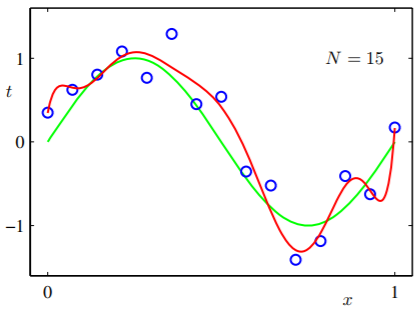
\includegraphics[width=0.5\columnwidth]{overfitting.png}
	\caption{Visualization of Over-fitting \cite{bishoptextbook}.}
	\label{overfittingpic}
\end{figure}

\paragraph{}
While there are many approaches to regularization neural networks, such as altering the networks error function to penalize for more complicated models or larger magnitude parameters, I chose one of the most straightforward and most easily interpretable methods: the early stopping approach. What this consists of is splitting data into a training and testing set, then training the model repeatedly on the training set, calculating the accuracy after each weight statemented with the testing set. After a set number of iterations, you select the model which produced the lowest training set accuracy, or similarly, the highest testing set accuracy. This prevents your model from over-fitting the training set.


\section{Results}
\paragraph{}
My data modeling of the data set consists of three main components. The first component was the general data clean up, which involved first obtaining the data, which I got from a Kaggle Repository. I then loaded the data and performed basic cleanup, which involved coercing strings to numeric types and converting categorical variables to dummy variables columns. I then subsetteds the data set to just contain entries from the U.S. elections. Finally, I dropped all non-numeric numeric columns, apart from the two categorical dummy variables (seat status and political party), to prepare for feeding into the model.


\begin{figure}[h]
	\centering
	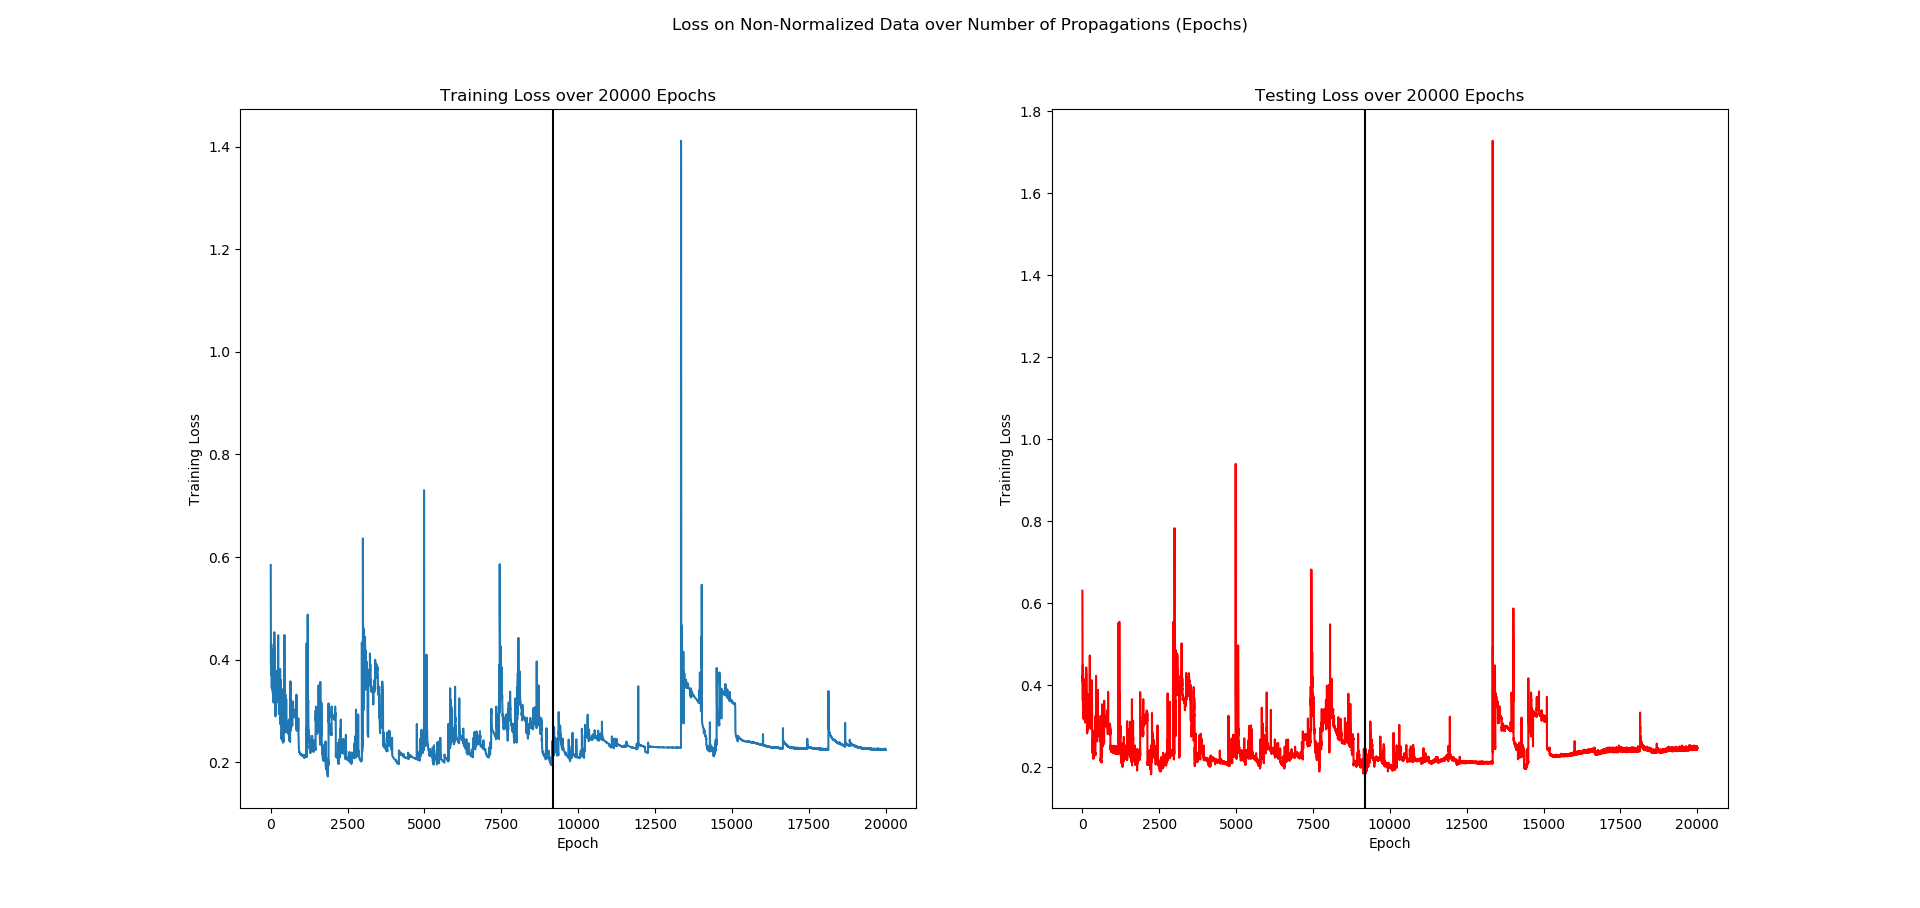
\includegraphics[width=1\columnwidth]{Simple_Loss_Non_Normalized_20000.png}
	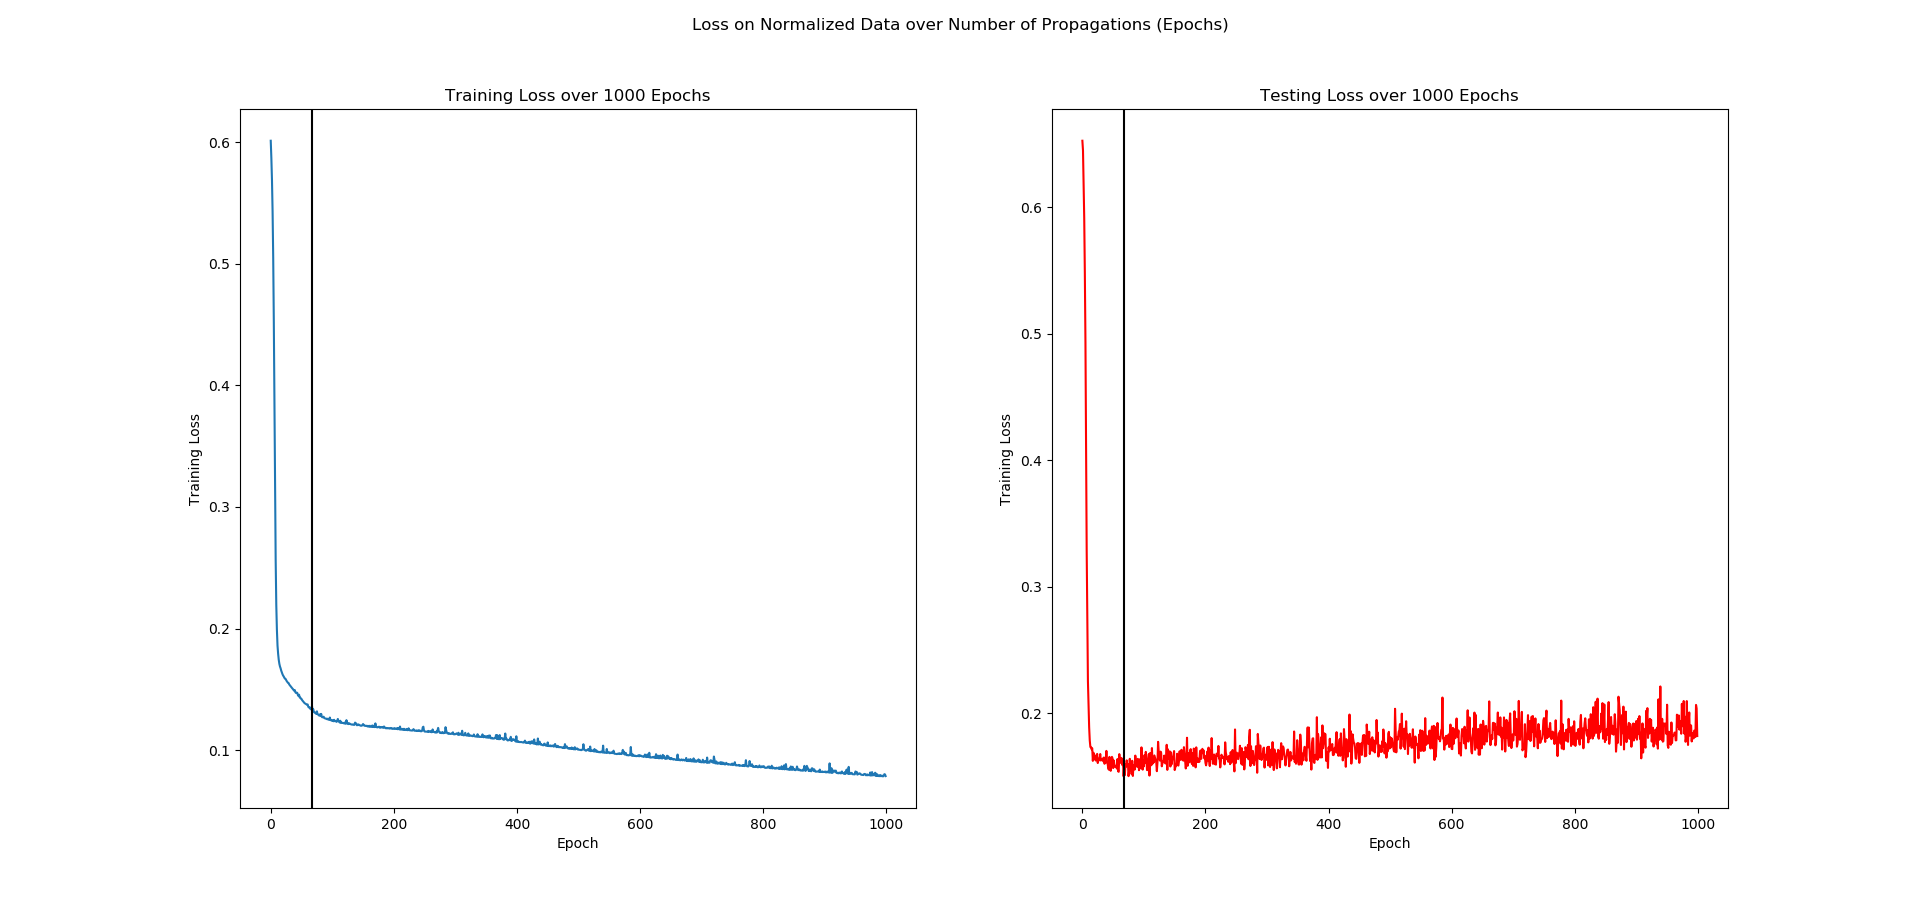
\includegraphics[width=1\columnwidth]{Simple_Loss_1000.png}
	\caption{Simple Model losses over Training Iterations (epochs)}
	\label{Simple_Model_Losses}
\end{figure}

\paragraph{}
The second portion of my analysis was to train two relatively simple models; each with one hidden layer one with the data input as is, and the other with the data normalized, both implementing the early stopping approach to regularization. I created a simple 90/10 training/testing data set split, to use both for the early stopping, and for an accuracy estimation. I then trained the normalized model on 2,000 iterations and attempted the same for the non-normalized model. The non-normalized model hadn't seemed to reach a smooth optimum, so I ran the process again with 20,000 iterations. As is shown in the Figure~\ref{Simple_Model_Losses}, which is both testing and training set loss over training iterations (epochs), the training process for the non-normalized model is much more noisier, and a testing accuracy optimum is reached after many more iterations than for the normalized data network. The vertical line in the charts are the testing set minimum loss over all the epochs, and thus the model that was returned from the process. Thus, I move forward using normalized data for my future models.


\paragraph{}
The network trained on normalized data had a simple testing accuracy of 95.8\%, while the network trained on non-normalized data had a simple testing set accuracy of 95.2\%. Neither of these models produced biased estimates, as they both misclassified an almost equal number in each class. Figure~\ref{Simple_Model_Classifications} shows the true election outcome next to predicted outcome and Figure~\ref{Simple_Model_Misclassifications} shows the misclassified data points.



\begin{figure}[h]
	\centering
	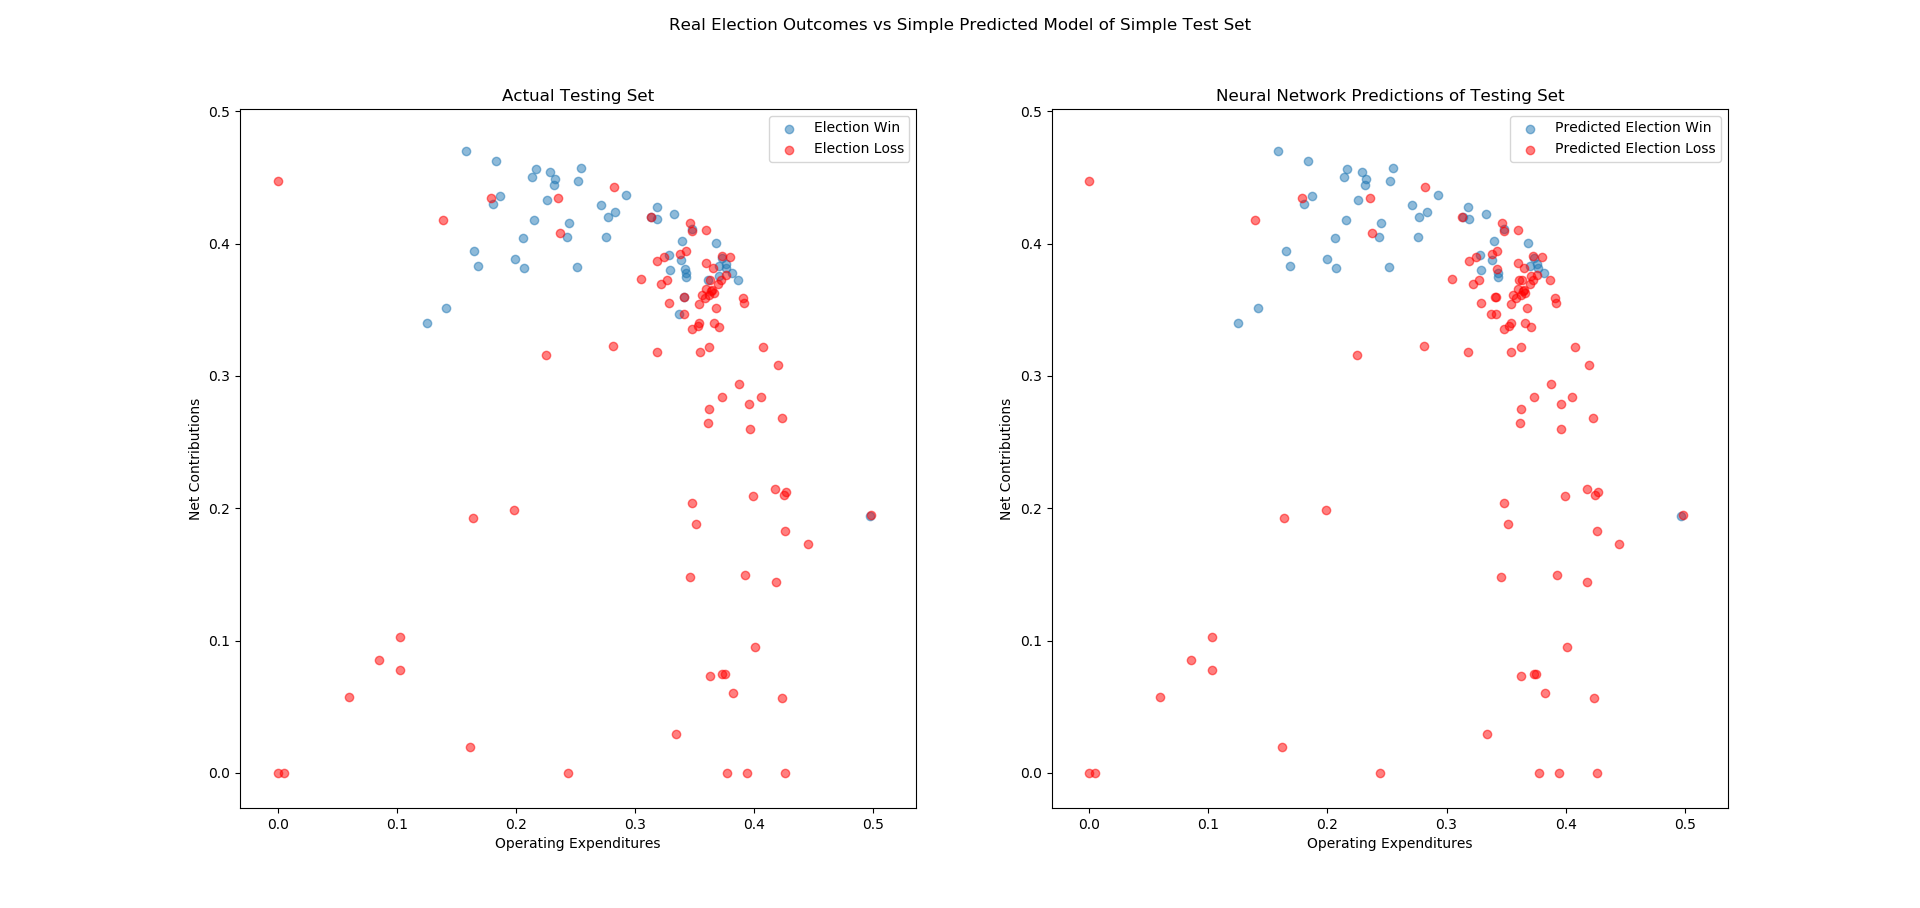
\includegraphics[width=1\columnwidth]{Simple_Classifications_1000.png}
	\caption{Simple Model Classifications over Two Predictors}
	\label{Simple_Model_Classifications}
\end{figure}

\begin{figure}[h]
	\centering
	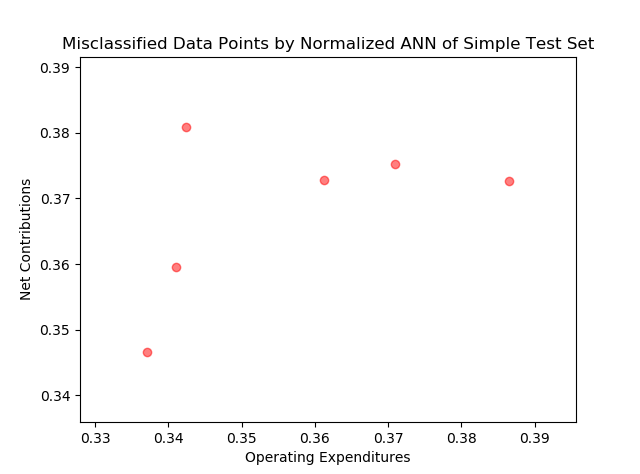
\includegraphics[width=0.8\columnwidth]{Simple_Misclassified_1000.png}
	\caption{Simple Model Misclassifications over over Two Predictors}
	\label{Simple_Model_Misclassifications}
\end{figure}


\paragraph{}
Before I moved forward to the cross validation, I trained another model with the normalized data, except with many more iterations. As displayed in Figure~\ref{Overtrained_Normalized_Model}, the training set loss converges 0, while the testing set loss explodes. This is a perfect representation of the need for regularization in neural networks.
\begin{figure}[h]
	\centering
	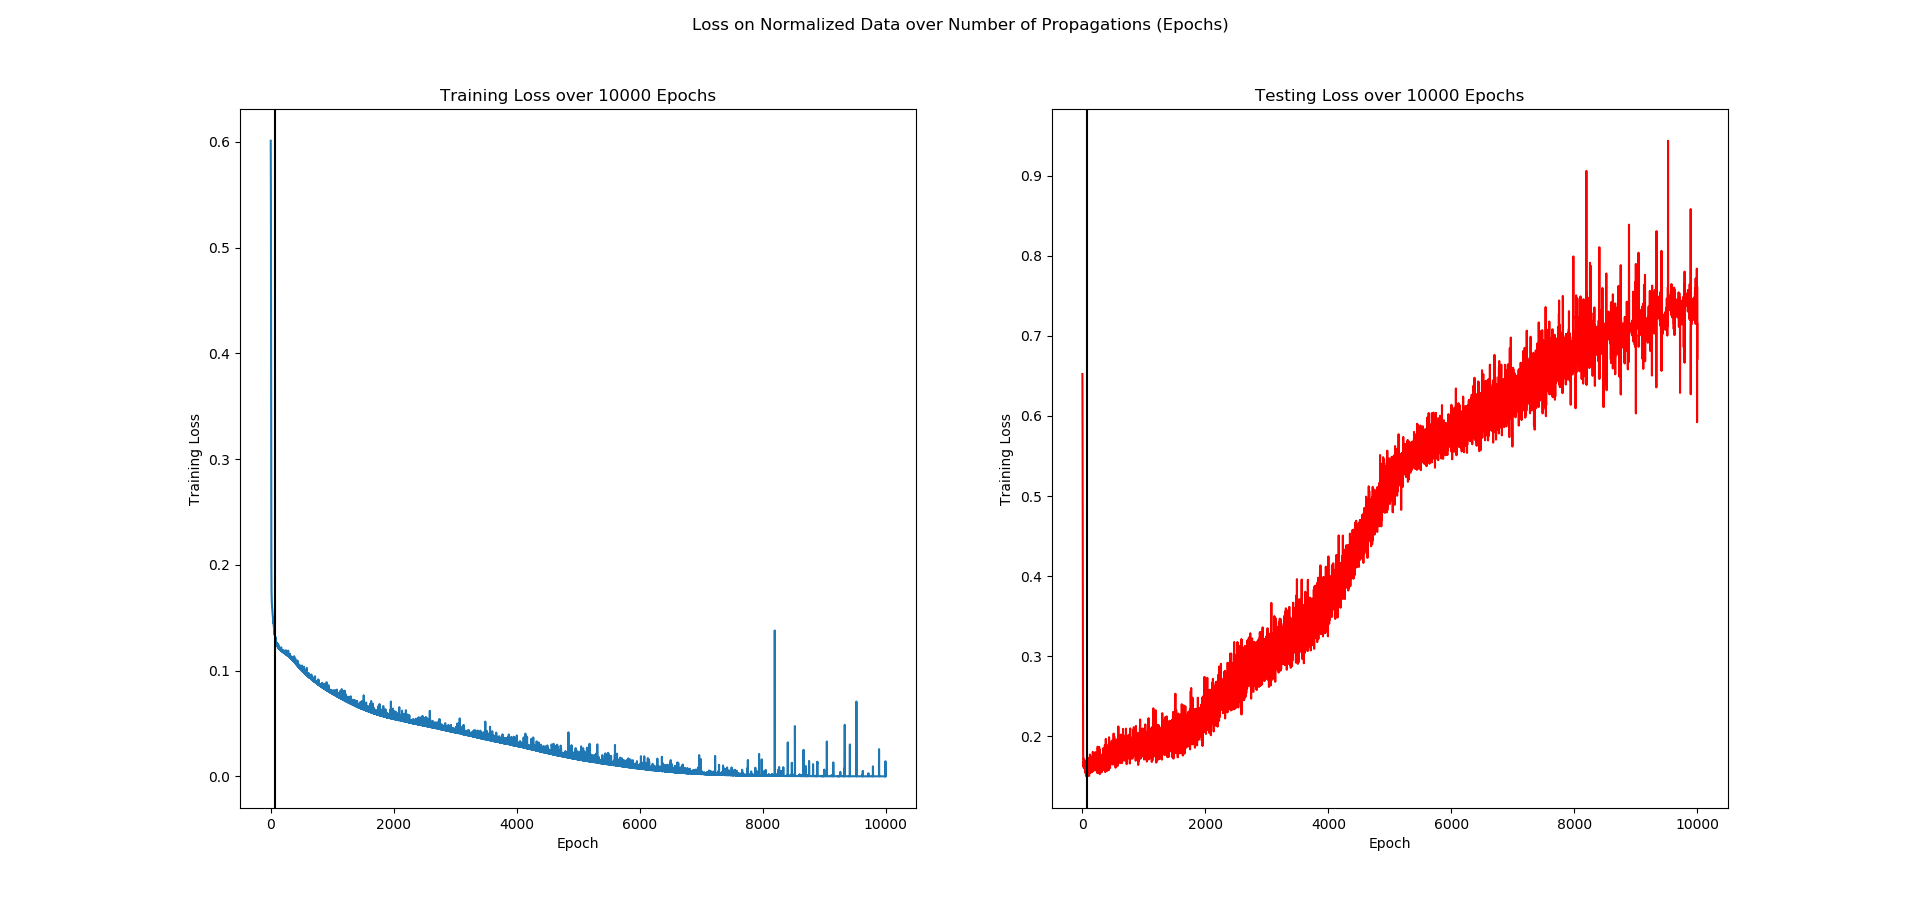
\includegraphics[width=1\columnwidth]{Simple_Loss_10000.png}
	\caption{Simple Normalized Model losses over 10,000 Training Iterations (epochs)}
	\label{Overtrained_Normalized_Model}
\end{figure}

\paragraph{}
The final portion of my analysis was to estimate the classification accuracy rates of several models through a 5 fold cross validation of the data set. To get an idea for different models, I trained models with sigmoidal activation functions with one, two, and three hidden layers, a single hidden layer model with ReLU activations, a single hidden layer model with the RMS Prop Optimizer, and a deeper network of 6 hidden layers with ReLU activations. The cross validated estimated classification accuracy and number of training iterations to reach optimal test set accuracy are displayed in Figure~\ref{CV_Folds}. One interesting observation from the visualization is that all models performed very similarly across the 5 folds, with really only two distinct outliers across the 30 data points. This is not incredibly surprising, as the models are fairly similar in construction. Another observation is that the second fold seemed to be the hardest to predict, also causing the most number of training iterations in the models. Finally, we can see that the deeper model needed many more iterations to reach an optimal value.

\paragraph{}
Finally, I display the cross validated estimated accuracy rates and average number of training iterations in Table~\ref{CV_Table}. With the exception of the single hidden layer ReLU, all models correctly classify about 95\% of testing data; quite similar to our previous analysis. Perhaps most interesting is the fact that the simplest of the models, the single hidden layer model with sigmoid activation functions, has the highest estimated accuracy rate. Since this data set was about 95\% linearly separable, this makes sense, as more complicated models again face the regularization issue.

\begin{figure}[h]
	\centering
	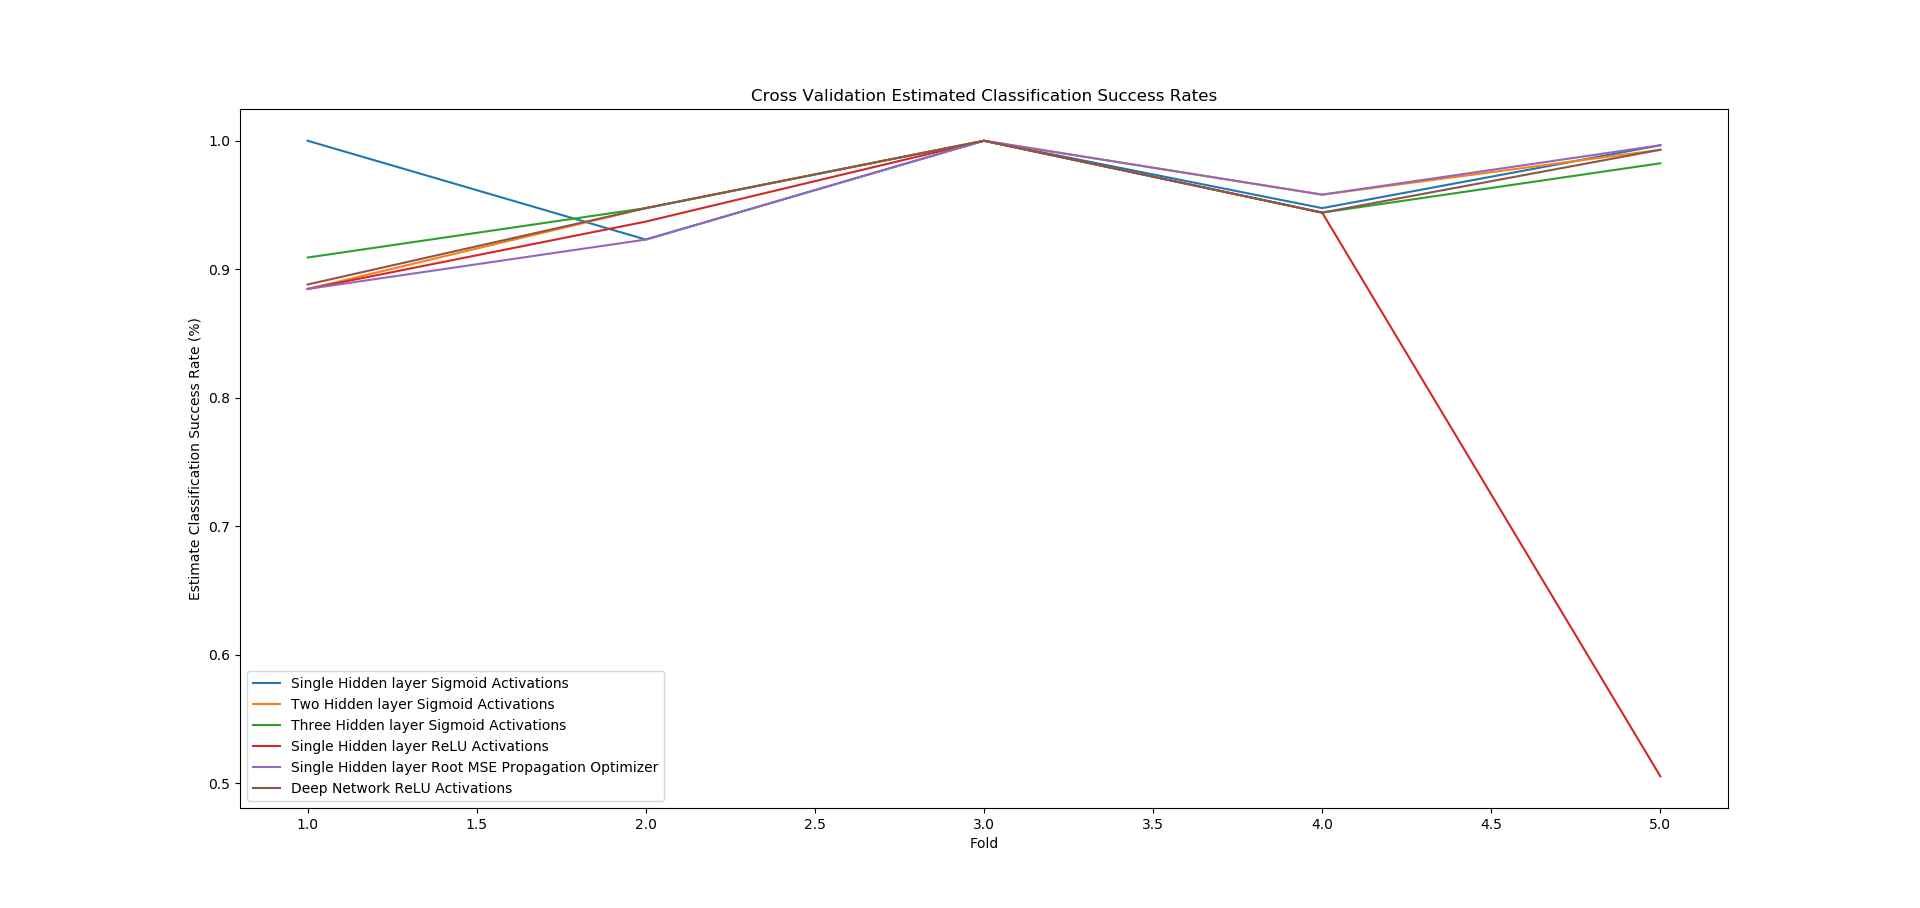
\includegraphics[width=1\columnwidth]{Cross_Validation_Error_Rates_Over_Folds.png}
	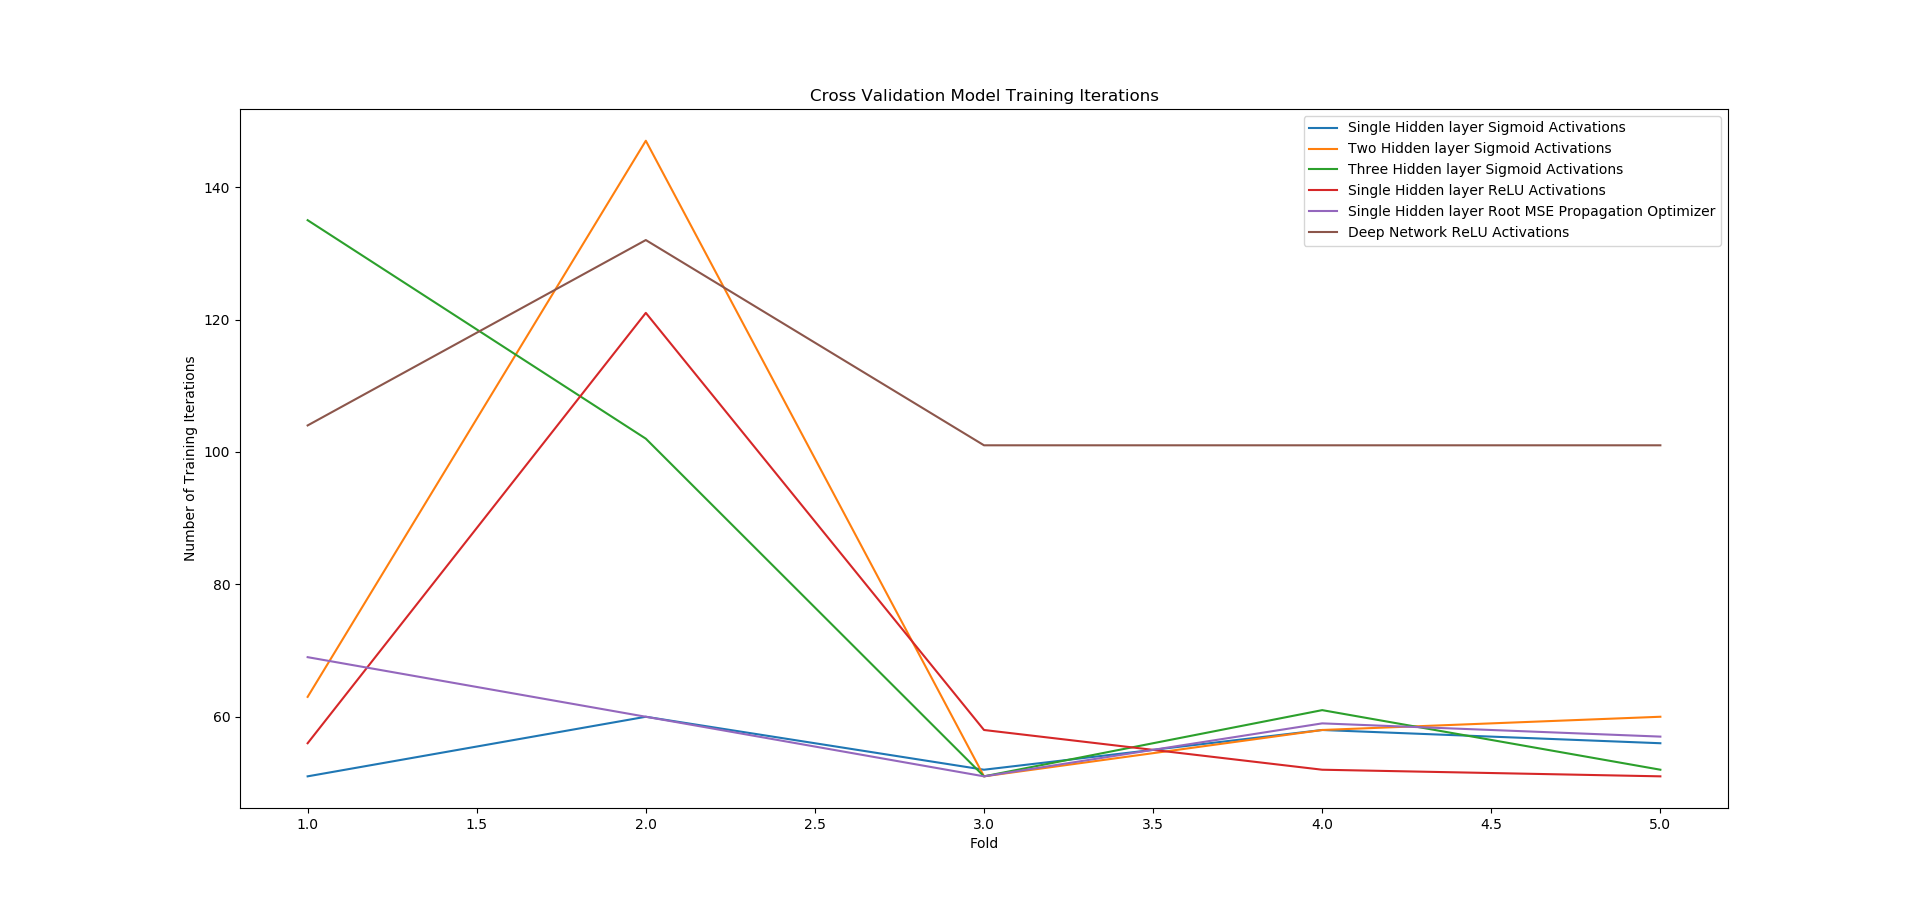
\includegraphics[width=1\columnwidth]{Cross_Validation_Training_Iterations_Over_Folds.png}
	\caption{Estimated Classification Accuracy Rates and Training Iterations for Selected Models}
	\label{CV_Folds}
\end{figure}


\paragraph{}

\begin{table}[h] % [h] forces the table to be output where it is defined in the code (it suppresses floating)
	\centering % Centre the table
	\begin{tabular}{l l l}
		\toprule
		\text{Model Type} & \text{CV Est. Accuracy Rate} & \text{Average Training Iterations} \\
		\midrule
		Single Hidden layer Sigmoid Activations & 97.34\% & 55.40\\
		Two Hidden layer Sigmoid Activations & 95.55\% & 75.80\\
		Three Hidden layer Sigmoid Activations & 95.66\% & 80.20\\
		Single Hidden layer ReLU Activations & 85.42\% & 67.60\\
		Single Hidden layer RMS Prop Optimizer & 95.24\% & 59.20\\
		Deep Network ReLU Activations & 95.45\% & 107.80\\
		\bottomrule
	\end{tabular}
	\caption{Cross Validated Success Rates and Average Training Iterations to reach minimum.}
	\label{CV_Table}
\end{table} 


\section{Conclusion}
\paragraph{}
As seen in our previous paper, 2016 U.S. House elections were incredibly predictable via several linear classification models, most getting around 95\% of the data correctly classified. When applying a radial basis kerneled support vector machine classifier to the data, we are able to get a 96.5\% cross validated estimated classification accuracy rate. When applying several relatively simple neural networks to the data, I was able to match that accuracy, and even exceed it by almost one percentage point with a just simple hidden layer sigmoid activation neural network.

\medskip
 
\begin{thebibliography}{9}

\bibitem{previouspaper} 
Campaign Finances in US House of Representatives Elections
\\\texttt{https://github.com/jaspermacnaughton/House-Elections-2016.}

\bibitem{opensecretsarticle}
Niv M. Sultan
\textit{Election 2016: Trump’s free media helped keep cost down, but fewer donors provided more of the cash}. 
https://www.opensecrets.org/news/2017/04/election-2016-trump-fewer-donors-provided-more-of-the-cash/

\bibitem{bishoptextbook} 
Christopher M. Bishop
\textit{Pattern Recognition and Machine Learning}. 
Springer Science Business Media, 2006.

\bibitem{kagglerepository} 
Kaggle: Campaign Finance versus Election Results
\\\texttt{https://www.kaggle.com/danerbland/electionfinance}

\bibitem{adam} 
Diederik P. Kingma and Jimmy Lei Ba
\textit{Adam: A Method for Stochastic Optimization}. 
https://arxiv.org/abs/1412.6980
The International Conference on Learning Representations


\end{thebibliography}


Source code maintained at: https://github.com/jaspermacnaughton/2016-House-Elections-Neural-Network

\end{document}
